\documentclass{beamer}

%
% Choose how your presentation looks.
%
% For more themes, color themes and font themes, see:
% http://deic.uab.es/~iblanes/beamer_gallery/index_by_theme.html
%
\mode<presentation>
{
  \usetheme{default}      % or try Darmstadt, Madrid, Warsaw, ...
  \usecolortheme{default} % or try albatross, beaver, crane, ...
  \usefonttheme{default}  % or try serif, structurebold, ...
  \setbeamertemplate{navigation symbols}{}
  \setbeamertemplate{caption}[numbered]
  \setbeamertemplate{footline}[page number]
  \setbeamercolor{frametitle}{fg=white}
  \setbeamercolor{footline}{fg=black}
} 

\usepackage[english]{babel}
\usepackage[utf8x]{inputenc}
\usepackage{tikz}
\usepackage{listings}
\usepackage{courier}
\usepackage{array}
\usepackage{ulem}

\xdefinecolor{darkblue}{rgb}{0.1,0.1,0.7}
\xdefinecolor{dianablue}{rgb}{0.18,0.24,0.31}
\definecolor{commentgreen}{rgb}{0,0.6,0}
\definecolor{stringmauve}{rgb}{0.58,0,0.82}

\lstset{ %
  backgroundcolor=\color{white},      % choose the background color
  basicstyle=\ttfamily\small,         % size of fonts used for the code
  breaklines=true,                    % automatic line breaking only at whitespace
  captionpos=b,                       % sets the caption-position to bottom
  commentstyle=\color{commentgreen},  % comment style
  escapeinside={\%*}{*)},             % if you want to add LaTeX within your code
  keywordstyle=\color{blue},          % keyword style
  stringstyle=\color{stringmauve},    % string literal style
  showstringspaces=false,
  showlines=true
}

\lstdefinelanguage{scala}{
  morekeywords={abstract,case,catch,class,def,%
    do,else,extends,false,final,finally,%
    for,if,implicit,import,match,mixin,%
    new,null,object,override,package,%
    private,protected,requires,return,sealed,%
    super,this,throw,trait,true,try,%
    type,val,var,while,with,yield},
  otherkeywords={=>,<-,<\%,<:,>:,\#,@},
  sensitive=true,
  morecomment=[l]{//},
  morecomment=[n]{/*}{*/},
  morestring=[b]",
  morestring=[b]',
  morestring=[b]"""
}

\newcommand\redsout{\bgroup\markoverwith{\textcolor{red}{\rule[0.5ex]{2pt}{1pt}}}\ULon}

\title[2016-07-18-julia]{Page of issues}
\author{Jim Pivsarski}
\institute{Princeton -- DIANA}
\date{July 18, 2016}

\begin{document}

\newcommand{\cfbox}[2]{%
    \colorlet{currentcolor}{.}%
    {\color{#1}%
    \fbox{\color{currentcolor}#2}}%
}

\logo{\pgfputat{\pgfxy(0.11, 8)}{\pgfbox[right,base]{\tikz{\filldraw[fill=dianablue, draw=none] (0 cm, 0 cm) rectangle (50 cm, 1 cm);}}}\pgfputat{\pgfxy(0.11, -0.6)}{\pgfbox[right,base]{\tikz{\filldraw[fill=dianablue, draw=none] (0 cm, 0 cm) rectangle (50 cm, 1 cm);}\includegraphics[height=0.99 cm]{diana-hep-logo.png}\tikz{\filldraw[fill=dianablue, draw=none] (0 cm, 0 cm) rectangle (4.9 cm, 1 cm);}}}}

%% \begin{frame}
%%   \titlepage
%% \end{frame}

\logo{\pgfputat{\pgfxy(0.11, 8)}{\pgfbox[right,base]{\tikz{\filldraw[fill=dianablue, draw=none] (0 cm, 0 cm) rectangle (50 cm, 1 cm);}\includegraphics[height=1 cm]{diana-hep-logo.png}}}}

% Uncomment these lines for an automatically generated outline.
%\begin{frame}{Outline}
%  \tableofcontents
%\end{frame}

\begin{frame}{Julia: a strange place in language space}
\vspace{0.25 cm}
\begin{center}
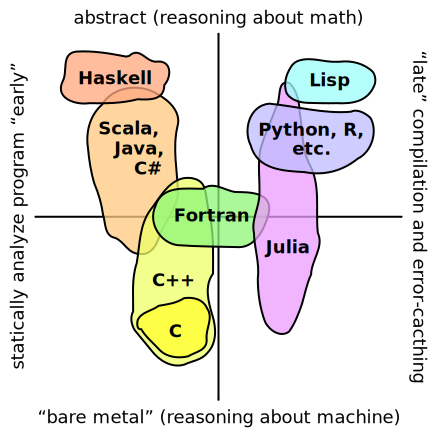
\includegraphics[width=0.75\linewidth]{language-grid.pdf}
\end{center}
\end{frame}

\begin{frame}{Julia is almost everything I wanted}
\vspace{0.5 cm}
{\bf My wish-list from last time:}

\begin{itemize}
\item define a subset of a \only<1>{well}\only<2>{\redsout{well}}-known syntax, such as \only<1>{Python}\only<2>{\redsout{Python} \textcolor{red}{Julia}}
\item that \only<1>{\cfbox{white}{JIT-compiles to CPU}}\only<2>{\cfbox{red}{JIT-compiles to CPU}}, GPU, and maybe FPGA
\item \only<1>{\cfbox{white}{that can be freely mixed with surrounding code}}\only<2>{\cfbox{red}{that can be freely mixed with surrounding code} \textcolor{red}{$\surd$}}
\item that is immutable, maybe total-functional\uncover<2>{\textcolor{red}{: check for Julia functions ending in ``!''}}
\item \only<1>{with special handling of Python's imperative statements and restrictive lambdas}\only<2>{\redsout{with special handling of Python's imperative statements and restrictive lambdas}}\uncover<2>{\textcolor{red}{: Julia syntax is expression-only and easily defines complex lambdas}}
\item using interval arithmetic as data types\uncover<2>{\textcolor{red}{: Julia's metaprogramming supports this kind of inspection}}
\item separate mathematics from performance annotations in CSS \uncover<2>{\textcolor{red}{Julia doesn't do this, but its metaprogramming would help build a demonstration project}}
\end{itemize}
\end{frame}

\begin{frame}{}
\vspace{1 cm}
\begin{center}
\Huge However\ldots
\end{center}
\end{frame}

\begin{frame}{Potential stumbling blocks for HEP analysts}
\vspace{0.4 cm}
\renewcommand{\arraystretch}{1.2}
\begin{tabular}{>{\raggedright}p{0.45\linewidth} >{\raggedright\arraybackslash}p{0.45\linewidth}}
{\bf Julia behavior} & {\bf HEP expectation} \\\hline
arrays range from $1$ to $N$ & $0$ to $N-1$ from C arrays, C++ vectors, and Python lists \\\hline
histogram (built-in {\tt \scriptsize hist()}) is exclusive on low edge and inclusive on high edge & inclusive on low edge and exclusive on high edge (HBOOK, PAW, ROOT, Numpy) \\\hline
multidimensional arrays are column-major & row-major C/C++, Numpy default, GPU \\\hline
no OOP-like fluent syntax: {\tt \scriptsize event.track(2).hit(12)} $\to$ {\tt \scriptsize hit(track(event, 2), 12)} & physicists have become accustomed to thinking in terms of objects \\\hline
{\tt \scriptsize elseif} (no space) & C/C++ {\tt \scriptsize else if}; Python {\tt \scriptsize elif}
\end{tabular}
\end{frame}

\begin{frame}{Potential issues for building large projects}
\vspace{0.4 cm}
\begin{itemize}
  \item Since everything is JIT-compiled, some errors are discovered only when they're encountered, such as {\tt \small UndefVarError}.

\vspace{0.2 cm}
Unit tests need to fill in for missing ``compiler checks,'' and it's hard to guarantee coverage of all potential uses (just like Python programming or C++ templates).

  \item {\tt \small Function} is not a parameterized type, so functions passed as arguments can't be constrained by method signature.

  \item Without methods in data structures (classes), the namespace fills up: I might think I'm defining a new function for my custom data structure, but I'm actually adding methods to a global function of the same name.

  \item Would need formal interfaces (contracts) to get an error if an implementation is incomplete.

  \item Do all packages need to be GitHub repositories ending in {\tt \small .jl}?
\end{itemize}
\end{frame}

\end{document}
